% Results from paper_q2_results/run_manifest.json; same saved 881 records.
\subsection{Within-Q2 Trajectories on the Same Corpus}
\label{sec:q2_trajectory_results}
We executed the rolling-window extension on the unchanged 881-record CSV and retained all 91 daily endpoints from April 1 through June 30, 2021. The non-overlapping monthly totals are 139 in April, 130 in May, and 134 in June, summing to the original 403 Q2 records. All Q2 windows satisfy the minimum support of five tickets, and none is a startup partial window because March history is retained. No synthetic tickets or additional quarters enter this analysis.

\textbf{Reproducibility and hierarchical correspondence.} The original per-ticket topic assignments from the Colab T4 GPU benchmark run were not preserved as a standalone CSV artifact, so this extension executes a documented shared-model fit on the exact same 881 records using MiniLM embeddings, 5D UMAP (15 neighbors, random seed 42), and HDBSCAN (minimum cluster size 16, minimum samples 5, unbounded EOM). On CPU, unbounded Excess-of-Mass (EOM) tree selection yielded 10 non-noise topics and 240 noise records over the full corpus (105 noise records in Q2). To avoid implying one-to-one numeric identity with Table~\ref{tab:topics_table}, we prefix this run's topic IDs with \textbf{R}. Crucially, cross-matching the medoid tickets and HDBSCAN condensed cluster tree reveals a clean hierarchical correspondence between the 14-topic benchmark (\texttt{T0}--\texttt{T13}) and the 10-topic rerun (\texttt{R0}--\texttt{R9}): eight topics map one-to-one (\texttt{T0}$\leftrightarrow$\texttt{R0}, \texttt{T1}$\leftrightarrow$\texttt{R2}, \texttt{T2}$\leftrightarrow$\texttt{R3}, \texttt{T5}$\leftrightarrow$\texttt{R4}, \texttt{T6}$\leftrightarrow$\texttt{R5}, \texttt{T7}$\leftrightarrow$\texttt{R6}, \texttt{T12}$\leftrightarrow$\texttt{R8}, \texttt{T13}$\leftrightarrow$\texttt{R9}), whereas unbounded EOM merged the three serialization/Arrow subsystems (\texttt{T8} multiprocessing pickle, \texttt{T9} Arrow memory/disk indexing, and \texttt{T4} PyArrow wheel bridge) into parent node \texttt{R1} ($N=298$) and merged \texttt{T10}+\texttt{T11} into \texttt{R7} ($N=56$). Applying bounded EOM ($m_{\max}=120$) on the exact same saved 5D UMAP manifold splits \texttt{R1} back into its constituent child clusters and recovers a 14-topic partition (Section~\ref{sec:ablations}).

\begin{figure*}[t]
    \centering
    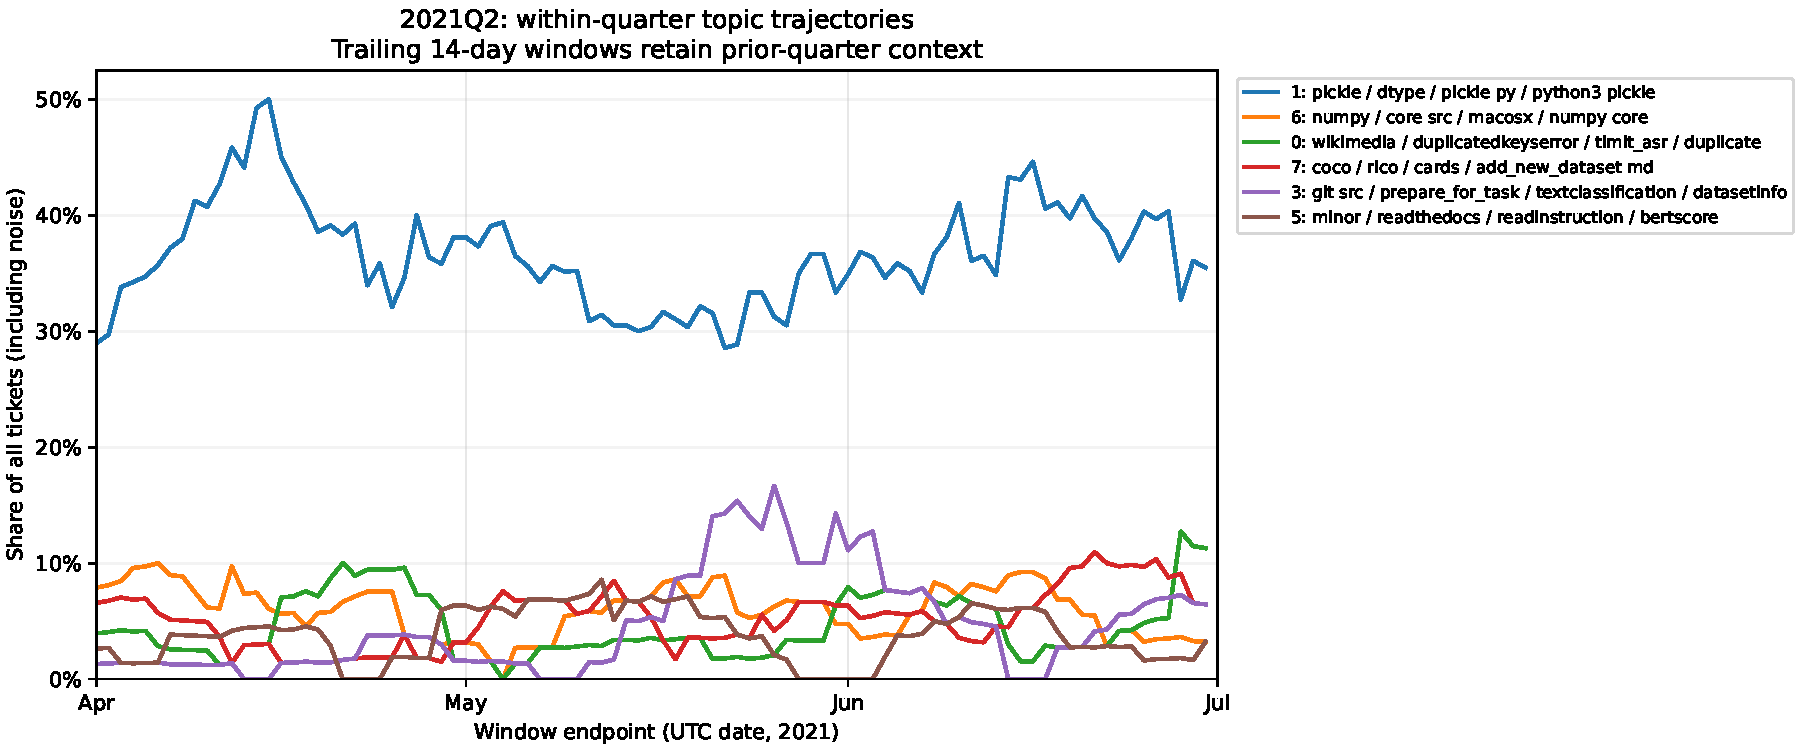
\includegraphics[width=0.98\textwidth]{paper_q2_results/topic_trajectories_2021Q2.pdf}
    \caption{Within-Q2 trajectories on the same incident corpus: daily 14-day trailing prevalence for the six most frequent non-noise Q2 topics in the documented rerun. The display covers April--June 2021; early-April windows retain March context. Noise is omitted from plotted curves but retained in every denominator. Numeric curve IDs belong only to the rerun, not the historical topic table.}
    \label{fig:q2_rolling_trajectories}
\end{figure*}

\begin{table}[t]
\centering
\small
\begin{tabular}{lrrr}
\toprule
\textbf{Rerun topic cue} & \textbf{Apr.} & \textbf{May} & \textbf{Jun.} \\
\midrule
R1: pickle / dtype & 41.73\% & 31.54\% & 40.30\% \\
R6: numpy / core & 5.04\% & 6.15\% & 5.97\% \\
R0: duplicate keys & 4.32\% & 4.62\% & 6.72\% \\
R7: coco / cards & 2.88\% & 6.15\% & 5.97\% \\
R3: task casting & 1.44\% & 9.23\% & 2.99\% \\
R5: documentation & 5.04\% & 3.08\% & 4.48\% \\
\bottomrule
\end{tabular}
\caption{Non-overlapping monthly shares of \emph{all} tickets in the same-data rerun. Denominators are 139, 130, and 134, respectively. These monthly shares differ from overlapping trailing-window shares. R-prefix IDs are local to this rerun.}
\label{tab:q2_monthly_prevalence}
\end{table}

Figure~\ref{fig:q2_rolling_trajectories} and Table~\ref{tab:q2_monthly_prevalence} expose timing that a single Q1-to-Q2 delta cannot resolve. The task-casting topic (R3) concentrated in May: its monthly share rose from 1.44\% in April to 9.23\% in May, then fell to 2.99\% in June. Its trailing prevalence peaked at 16.67\% on May 26. The duplicate-key topic (R0) showed a later concentration, reaching a trailing peak of 12.73\% on June 28; its monthly share increased from 4.32\% in April to 6.72\% in June. These patterns describe temporal concentration, not evidence of a deployment-induced outage or confirmed remediation.

The large pickle/dtype parent topic (R1) illustrates why endpoint change should not be interpreted as monotonic growth: it began Q2 at 28.95\%, peaked at 50.00\% on April 15, and ended at 35.48\%, yet its least-squares slope across all Q2 endpoints was slightly negative ($-0.058$ percentage points per week, non-parametric Mann--Kendall $\tau_{\text{MK}} = +0.0056, p = 0.937$) \cite{mann1945nonparametric}. By contrast, task casting (R3) exhibits a strong positive monotonic trajectory ($\tau_{\text{MK}} = +0.3589$, raw $p = 5.9 \times 10^{-7}$, $+0.521$ pp/week), while column operations (R2, $\tau_{\text{MK}} = -0.5788$) and NumPy/checksum issues (R6, $\tau_{\text{MK}} = -0.1600$) exhibit declining trajectories. Endpoint net change, peak timing, and whole-quarter slope summarize different aspects of a fluctuating curve. Because R1 merges three child serialization and Arrow/I/O clusters in the unbounded EOM fit, it represents a macro-subsystem rather than a single atomic failure mode.

% Both comparisons reuse paper_q2_results/topic_assignments.csv unchanged.
\subsubsection{Q1-Referenced Trajectory Comparisons}
\label{sec:q1_q2_comparisons}
We evaluated both subtraction options using exactly the same saved rerun assignments, with \emph{no additional topic-model fit}. The Q1 baseline contains 478 tickets and the Q2 target contains 403 tickets. Option~1 has 91 comparable Q2 endpoints. Option~2 has 77 comparable ordinal-day pairs (days 14--90): 13 target days are excluded because the corresponding Q1 startup windows are partial, and Q2 day 91 has no Q1 endpoint. All denominators include noise. Differences are reported in percentage points (pp), not relative percent changes.

\begin{figure*}[t]
    \centering
    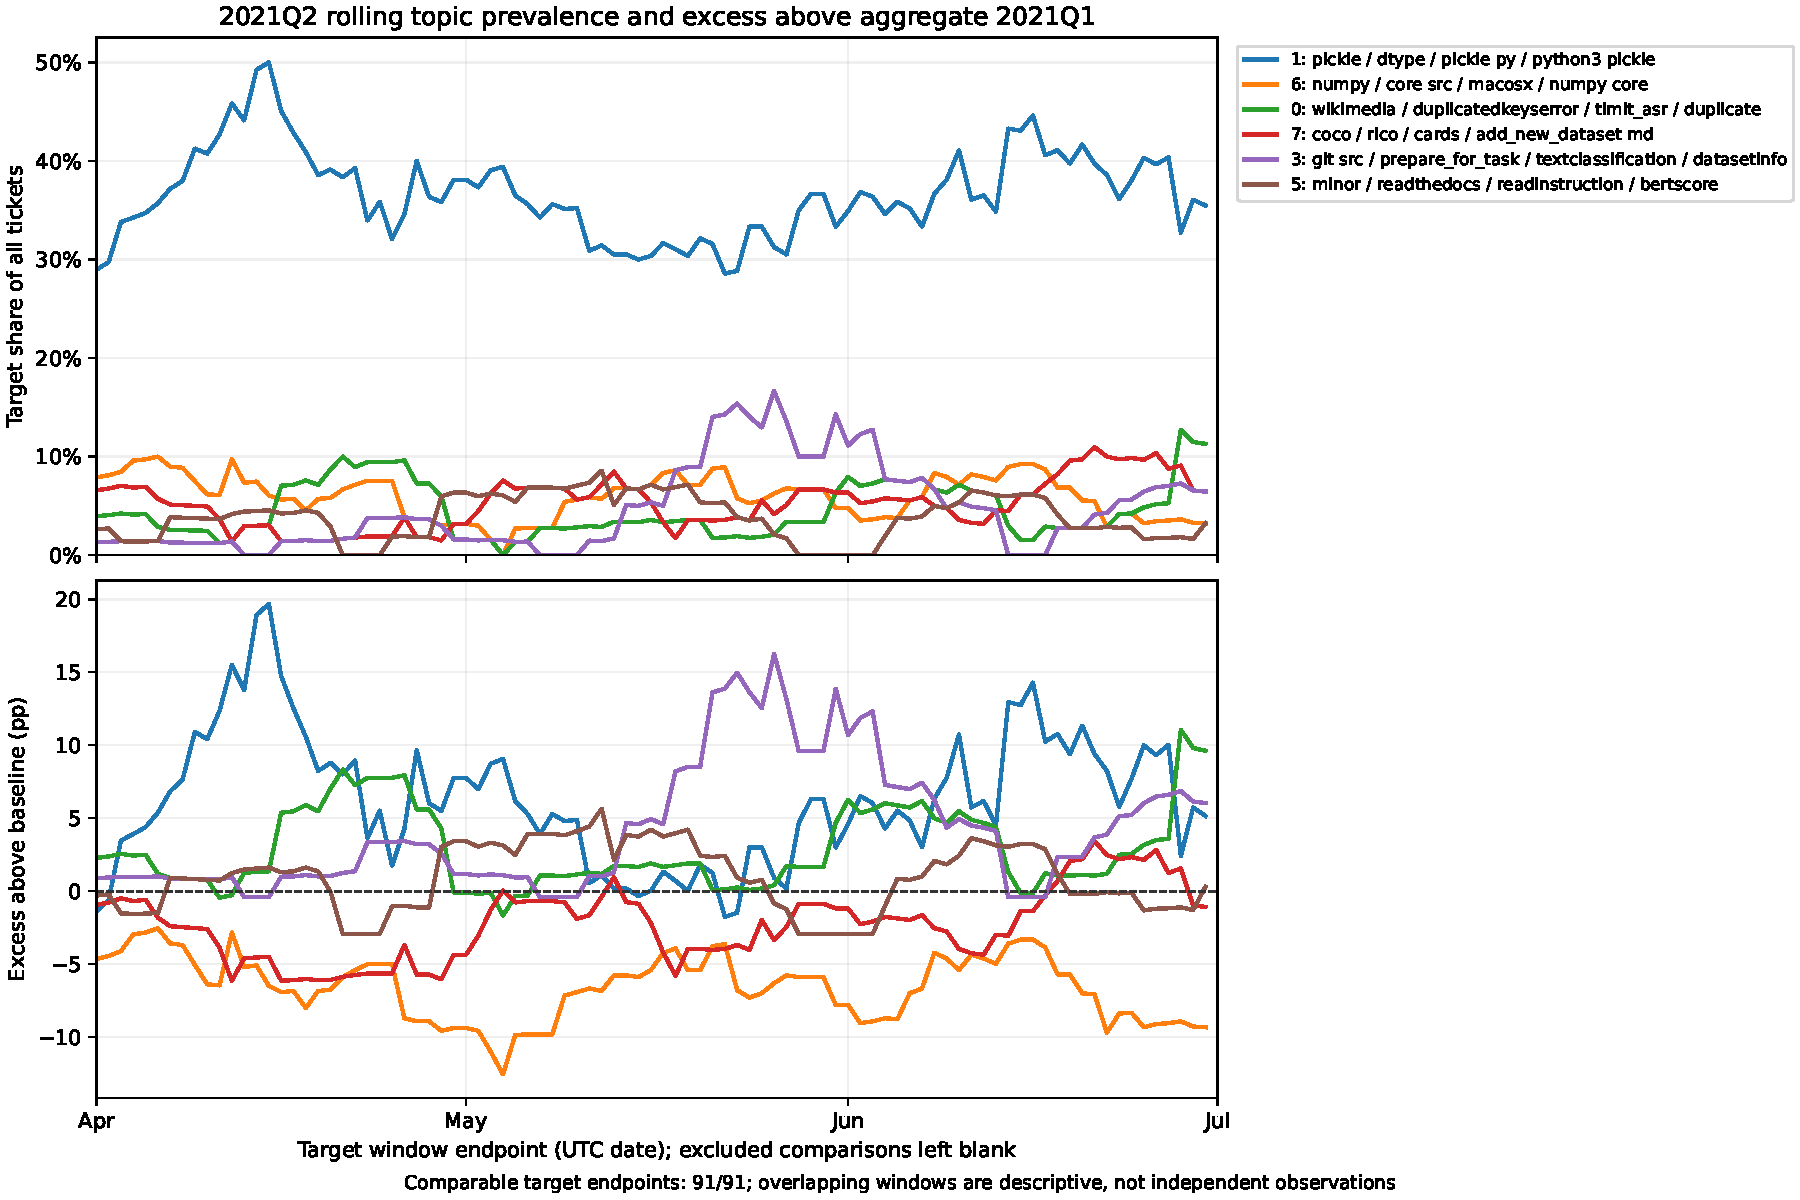
\includegraphics[width=0.98\textwidth]{paper_q2_results/comparisons/baseline_excess_2021Q2_vs_2021Q1.pdf}
    \caption{Option~1: actual Q2 rolling prevalence (top) and excess above the overall Q1 prevalence of the same topic (bottom). The baseline uses original Q1 counts, not the mean of overlapping Q1 windows. Positive values indicate an elevated share relative to Q1; the dashed zero line marks baseline parity. The six non-noise topics are selected by Q2 counts; all denominators retain noise. IDs belong only to the documented same-data rerun.}
    \label{fig:q1_baseline_excess}
\end{figure*}

\begin{figure*}[t]
    \centering
    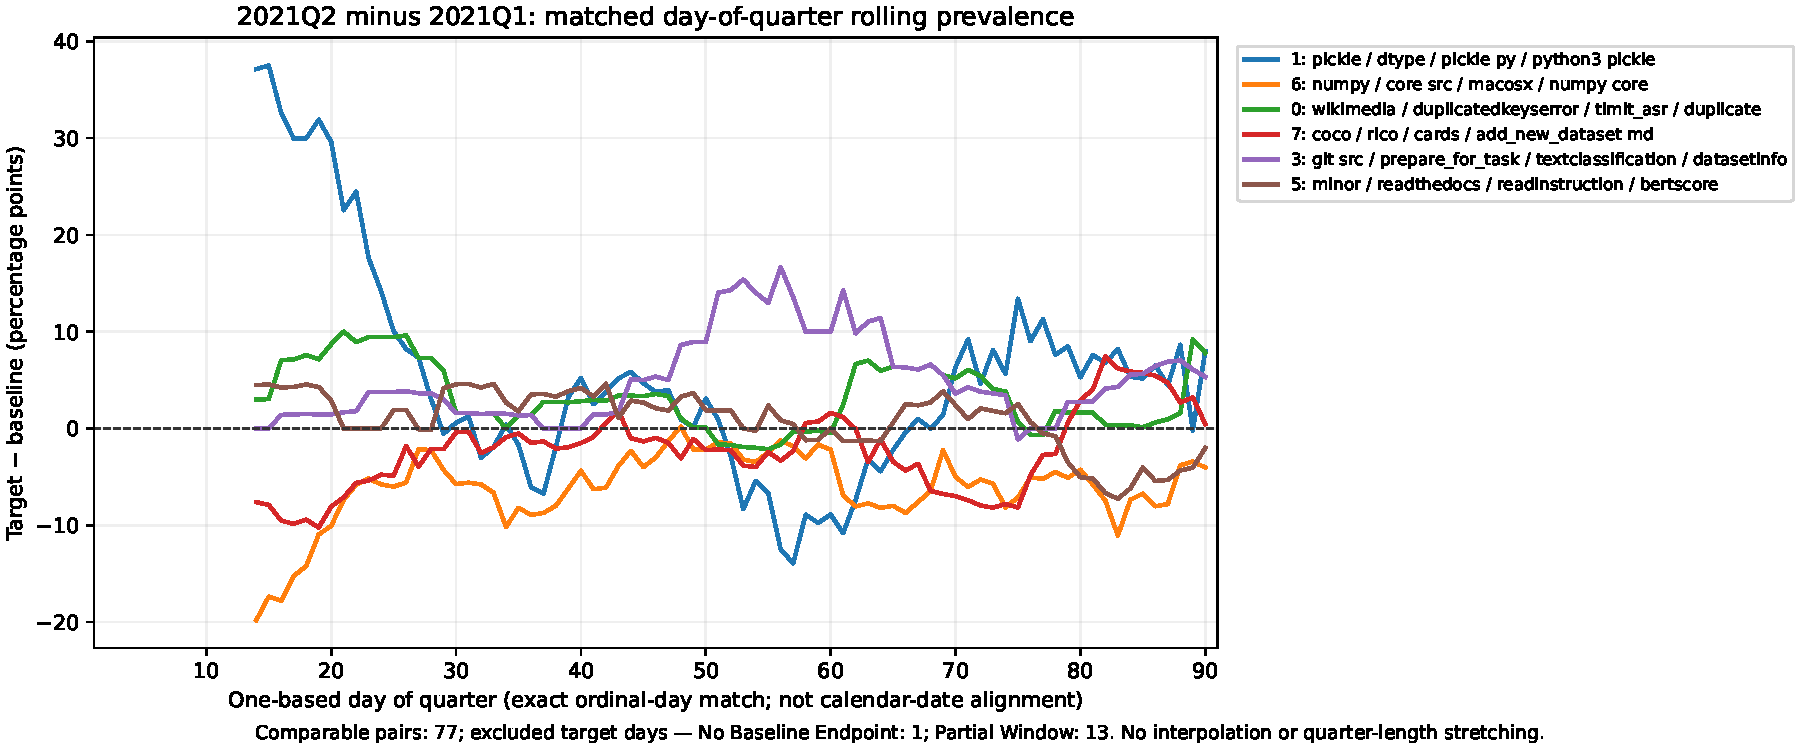
\includegraphics[width=0.98\textwidth]{paper_q2_results/comparisons/aligned_difference_2021Q2_vs_2021Q1.pdf}
    \caption{Option~2: Q2 rolling prevalence minus Q1 rolling prevalence at the same one-based day of quarter. Both windows must be full-length and supported. The 90/91-day timelines are not stretched or interpolated; Q1 startup days 1--13 and unmatched Q2 day 91 have no difference estimate. Ordinal-day alignment is exploratory and does not control for weekdays, holidays, or release events.}
    \label{fig:q1_q2_aligned_difference}
\end{figure*}

\begin{table}[t]
\centering
\small
\begin{tabular}{lrrr}
\toprule
\textbf{Rerun cue} & \textbf{Q1 share} & \textbf{Mean $E$} & \textbf{Mean $D$} \\
\midrule
R1: pickle / dtype & 30.33\% & +6.29 & +5.27 \\
R0: duplicate keys & 1.67\% & +2.92 & +3.34 \\
R3: task casting & 0.42\% & +4.26 & +4.98 \\
R6: numpy / core & 12.55\% & $-6.56$ & $-6.14$ \\
\bottomrule
\end{tabular}
\caption{Descriptive mean differences in pp: $E$ averages 91 Q2 endpoints relative to the overall Q1 baseline; $D$ averages 77 exact ordinal-day pairs. These are different reference constructions and endpoint sets, not independent estimates of the same quantity. R-prefix IDs identify the saved rerun.}
\label{tab:q1_q2_comparisons}
\end{table}

\textbf{Elevation relative to Q1.} Figure~\ref{fig:q1_baseline_excess} shows that the task-casting topic (R3) exceeds its Q1 baseline of 0.42\% at 80 of 91 Q2 endpoints. Its maximum excess is +16.25 pp on May 26, and its mean excess is +4.26 pp. The NumPy/core topic (R6), by contrast, remains below its 12.55\% Q1 baseline at \emph{every} Q2 endpoint, with mean excess $-6.56$ pp. Thus a nonzero absolute Q2 trajectory need not indicate a new elevation over the earlier baseline. These findings describe shifts in share; they do not by themselves establish causes or remediation.

\textbf{Timing relative to the earlier curve.} Figure~\ref{fig:q1_q2_aligned_difference} offers a different reference: the R3 peak on Q2 day 56 (May 26) is +16.67 pp above Q1 day 56 (February 25). For R0, the largest excess above the aggregate Q1 baseline occurs on June 28 (+11.05 pp), whereas its largest paired difference occurs on day 21, April 21 versus January 21 (+10.00 pp). The dates differ because the earlier-quarter curve varies over time; replacing a constant baseline with an ordinal-day reference changes the question being asked.

The broad pickle/dtype topic (R1) has mean excess +6.29 pp but mean aligned difference +5.27 pp. Its peak on April 15 is +19.67 pp above the overall Q1 baseline, yet +37.50 pp above the January 15 rolling estimate. This larger paired contrast partly reflects a low value at that \emph{particular} Q1 position, not a stronger causal effect. Table~\ref{tab:q1_q2_comparisons} reports both summaries without treating them as interchangeable.

Both comparisons are retrospective and descriptive. Overlapping windows are dependent, and both quarter positions and period support can affect the differences. We retain the aggregate-baseline plot as the more direct operational reference and the aligned-curve subtraction as an exploratory timing comparison; neither is a significance test, incident-rate estimate per day, or proof of a regression.


The implementation can focus on any quarter present in the assignments, but these paper results concern only \textbf{Q2 2021 on the existing dataset}. The fresh-fit trajectory results are a separate descriptive extension; exact within-Q2 trajectories for the historical 14-topic solution would require recovering its per-ticket assignments or recreating and verifying that precise model fit.
